% ====================================================================
%+
% SECTION:
%    section-name.tex  % eg lenstimedelays.tex
%
% CHAPTER:
%    chapter.tex  % eg cosmology.tex
%
% ELEVATOR PITCH:
%    Explain in a few sentences what the relevant discovery or
%    measurement is going to be discussed, and what will be important
%    about it. This is for the browsing reader to get a quick feel
%    for what this section is about.
%
% COMMENTS:
%
%
% BUGS:
%
%
% AUTHORS:
%    Phil Marshall (@drphilmarshall)  - put your name and GitHub username here!
%-
% ====================================================================

\section{AGN Selection and Census}
\def\secname{\chpname:census}\label{sec:\secname}

\credit{ohadshemmer},
\credit{nielbrandt},
\credit{GordonRichards},
\credit{AstroVPK},
\credit{ScottAnderson},
{\it and others to follow}

% This individual section will need to describe the particular
% discoveries and measurements that are being targeted in this section's
% science case. It will be helpful to think of a ``science case" as a
% ``science project" that the authors {\it actually plan to do}. Then,
% the sections can follow the tried and tested format of an observing
% proposal: a brief description of the investigation, with references,
% followed by a technical feasibility piece. This latter part will need
% to be quantified using the MAF framework, via a set of metrics that
% need to be computed for any given observing strategy to quantify its
% impact on the described science case. Ideally, these metrics would be
% combined in a well-motivated figure of merit. The section can conclude
% with a discussion of any risks that have been identified, and how
% these could be mitigated.

% A short preamble goes here. What's the context for this science
% project? Where does it fit in the big picture?

%\new{From Phil: Large samples of LSST AGN will provide high precision constraints
%on  galaxy evolution models. The science yield will be maximized  by
%increasing the sample size; the accuracy with which the selection
%function is known may also be important. }

The primary goal for AGN science is to maximize the discovery of AGN
with the LSST and construct the largest possible inventory of sources
spanning the widest possible ranges in the redshift-luminosity parameter
space. This, in turn, will provide high-precision constraints on galaxy
evolution models as well as on various cosmological science cases,
such as quasar clustering, the highest redshift quasars, and
strong gravitational lensing.

% --------------------------------------------------------------------

\subsection{Target measurements and discoveries}
\label{sec:\secname:targets}

% Describe the discoveries and measurements you want to make.

% Now, describe their response to the observing strategy. Qualitatively,
% how will the science project be affected by the observing schedule and
% conditions? In broad terms, how would we expect the observing strategy
% to be optimized for this science?

%\new{From Phil: Our target measurements will be inferences of galaxy evolution
%model  parameters, from a joint analysis with the host galaxy
%properties. As an initial proxy, we focus on the quasar luminosity
%function -- and  as a first step towards that, the number counts.}

It is expected that $\approx 10^7 - 10^8$ AGNs will be selected in the
main LSST survey using a combination of criteria, split broadly into
four categories: colors, astrometry, variability, and multiwavelength
matching with other surveys. The LSST observing strategy will affect
mostly the first three of these categories as described further below.

{\bf Colors:} The LSST observing strategy will determine the depth in
each band, as a function of position on the sky, and will thus affect
the color selection of AGNs. This will eventually determine the AGN
$L-z$ distribution and, in particular, may affect the identification
of quasars at $z\gtsim 6$ if, for example, $Y$-band exposures will
not be sufficiently deep.

{\bf Variability:} AGNs can be effectively distinguished from (variable)
stars, and from quiescent galaxies, by exhibiting certain characteristic
variability patterns (e.g., \citet{ButlerandBloom2011}). Picking the
right cadence can increase the effectiveness of AGN selection.

%Non-uniform
%sampling may ``contaminate'' the variability signal of AGN candidates.

{\bf Astrometry:} AGNs will be selected among sources having zero
proper motion, within the uncertainties. The LSST cadence may affect
the level of this uncertainty in each band, and may therefore affect
the ability to identify (mostly fainter) AGN.
%
Differential chromatic refraction (DCR), making use of the astrometric
offset a source with emission lines has with respect to a source with
a featureless power-law spectrum, can help in the selection of AGNs
and in confirming their photometric redshifts
\citep{KaczmarczikEtal2009}. The DCR effect is more pronounced at
higher airmasses. Therefore, it could be advantageous to have at least one
visit, per source, at airmass greater than about 1.4. AGN selection
and photometric redshift confirmation may be affected since the LSST
cadence will affect the airmass distribution, in each band, for each
AGN candidate.

The most critical measurement for the AGN census is having a reliable
and precise redshift for each source, obtained both from a photometric
and an astrometric redshift.

% Ideas for Metrics:
% detection - how many can LSST detect based on the luminosity function
% (depends on the depth in each band for single epoch and coadd)
% (how will this change with each DR)? @ohadshemmer

% classification - How many of these will we actually classify as quasars?
% non-simultaneous colors. variability of QSOs (how does depend on
% cadence/baseline/seasonal gaps?)

% --------------------------------------------------------------------

\subsection{Metrics}
\label{sec:\secname:metrics}

Quantifying the response via MAF metrics: definition of the metrics,
and any derived overall figure of merit.

The following are most important for the AGN census:

1) Determine the mean (averaged across the sky) uncertainty on astrometric
redshifts derived from DCR as a function of airmass, image quality, and
limiting magnitude. These uncertainties should be compared to the
corresponding uncertainties on the photomteric redshift.

2) Estimate the number of quasars at $z>6$ that LSST can discover
during a single visit as well as the entire survey and verify that
these numbers do not fall short of the original predictions. This
requires computing the limiting $Y$-band magnitude, averaged
across the sky for the nominal OpSim.

3) Assess the effect of non-simultaneous colors on AGN selection. Each
source would be represented as an ellipse in color-color space. The aim
is to assess the sizes of the ellipses and how these sizes could be
minimized by perturbing the current cadence.

4) Estimate the number of low-luminosity AGN (LLAGN) that can be
identified during the entire survey.

% --------------------------------------------------------------------

\subsection{OpSim Analysis}
\label{sec:\secname:analysis}

OpSim analysis: how good would the default observing strategy be, at
the time of writing for this science project?

1) For assessing the limitations of DCR, need to obtain from OpSim
the current maximal airmasses for each band, and the associated
image quality and limiting magnitude. Convert this output into
the mean and spread of the uncertainty on the astrometric redshifts.
Need to fold the astrometric redshift estimation from DCR into MAF.
Check the implications of higher airmasses and limiting magnitudes
on the ability to obtain more accurate and precise astrometric redshifts.

2) For predicting the number of detected $z>6$ quasars
%Compare this magnitude to the
%one required for identifying $\geq1000$ quasars at $z\geq6$.
the current enigma\_1189 OpSim gives a single-epoch 5-sigma depth
$Y=22.36$ mag, and for the final co-added 5-sigma depth it is $Y=24.4$.
These limits are correspondingly deepered than the original predictions
(see plot).
% (See the AAS poster from 2013: http://www.lsst.org/sites/default/files/221-RC-247.10-AAS_shemmer.pptx.pdf).

%\begin{figure}
%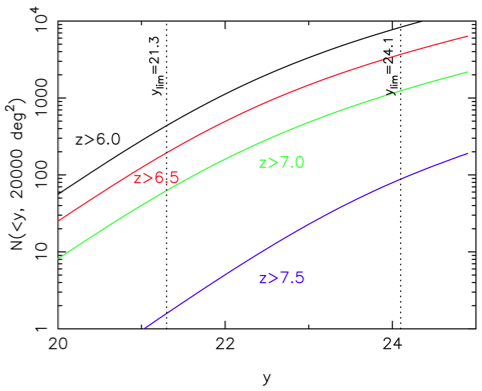
\includegraphics[width=5.0in]{figs/agn/zgt6_figure_AAS_2013.tiff}
%\caption{Number of quasars at $z>6$ that LSST is expected to discover
%based on $Y$-band limiting magnitude in a single epoch (entire survey)
%marked by the first (second) dotted line from the left.}
%\label{fig:zgt6}
%\end{figure}

3) Simulate the amplitudes of the uncertainties in color-color space and how
these depend on the cadence.

4) Maximizing the number of LLAGN - depends mostly on effective variability selection
(C-ARMA). More work needed here...

% --------------------------------------------------------------------

\subsection{Discussion}
\label{sec:\secname:discussion}

Discussion: what risks have been identified? What suggestions could be
made to improve this science project's figure of merit, and mitigate
the identified risks?


% ====================================================================

\navigationbar
